\documentclass[letterpaper]{article}
\usepackage[submission]{aaai2027}
\usepackage{times}
\usepackage{helvet}
\usepackage{courier}
\usepackage[hyphens]{url}
\usepackage{graphicx}
\usepackage{booktabs}
\usepackage{microtype}
\usepackage{amsmath}
\usepackage{amssymb}
\usepackage{natbib}
\usepackage{caption}
\frenchspacing
\setlength{\pdfpagewidth}{8.5in}
\setlength{\pdfpageheight}{11in}
\urlstyle{rm}
\def\UrlFont{\rm}

\pdfinfo{
/TemplateVersion (2027.1)
}

\setcounter{secnumdepth}{0}

\title{Supplementary Material: Graph-Guided Mixture-of-Experts \\
for Unified Multimodal Mental Health Assessment}

\author{
Anonymous Authors
}
\affiliations{
}

\begin{document}

\maketitle

\section{Experimental Pipeline Overview}

The central empirical question of the main paper is the graph-routing investigation. To isolate its effect, we compare five graph-routing ablation variants (V0--V4) against non-graph baselines. When initial results showed no improvement on DAIC/MOSEI and degradation on FI personality, we deployed a homophily diagnostic comparing real graph edges against random pairing, alongside targeted fixes including a $K$-sensitivity sweep ($K=5, 10, 15, 20$) and learning a per-task $\lambda$ weight instead of fixing it at 0.5. These diagnostics confirmed that graph routing does not help in this setting because the required signal is either absent or unused.

\begin{figure*}[htbp]
\centering
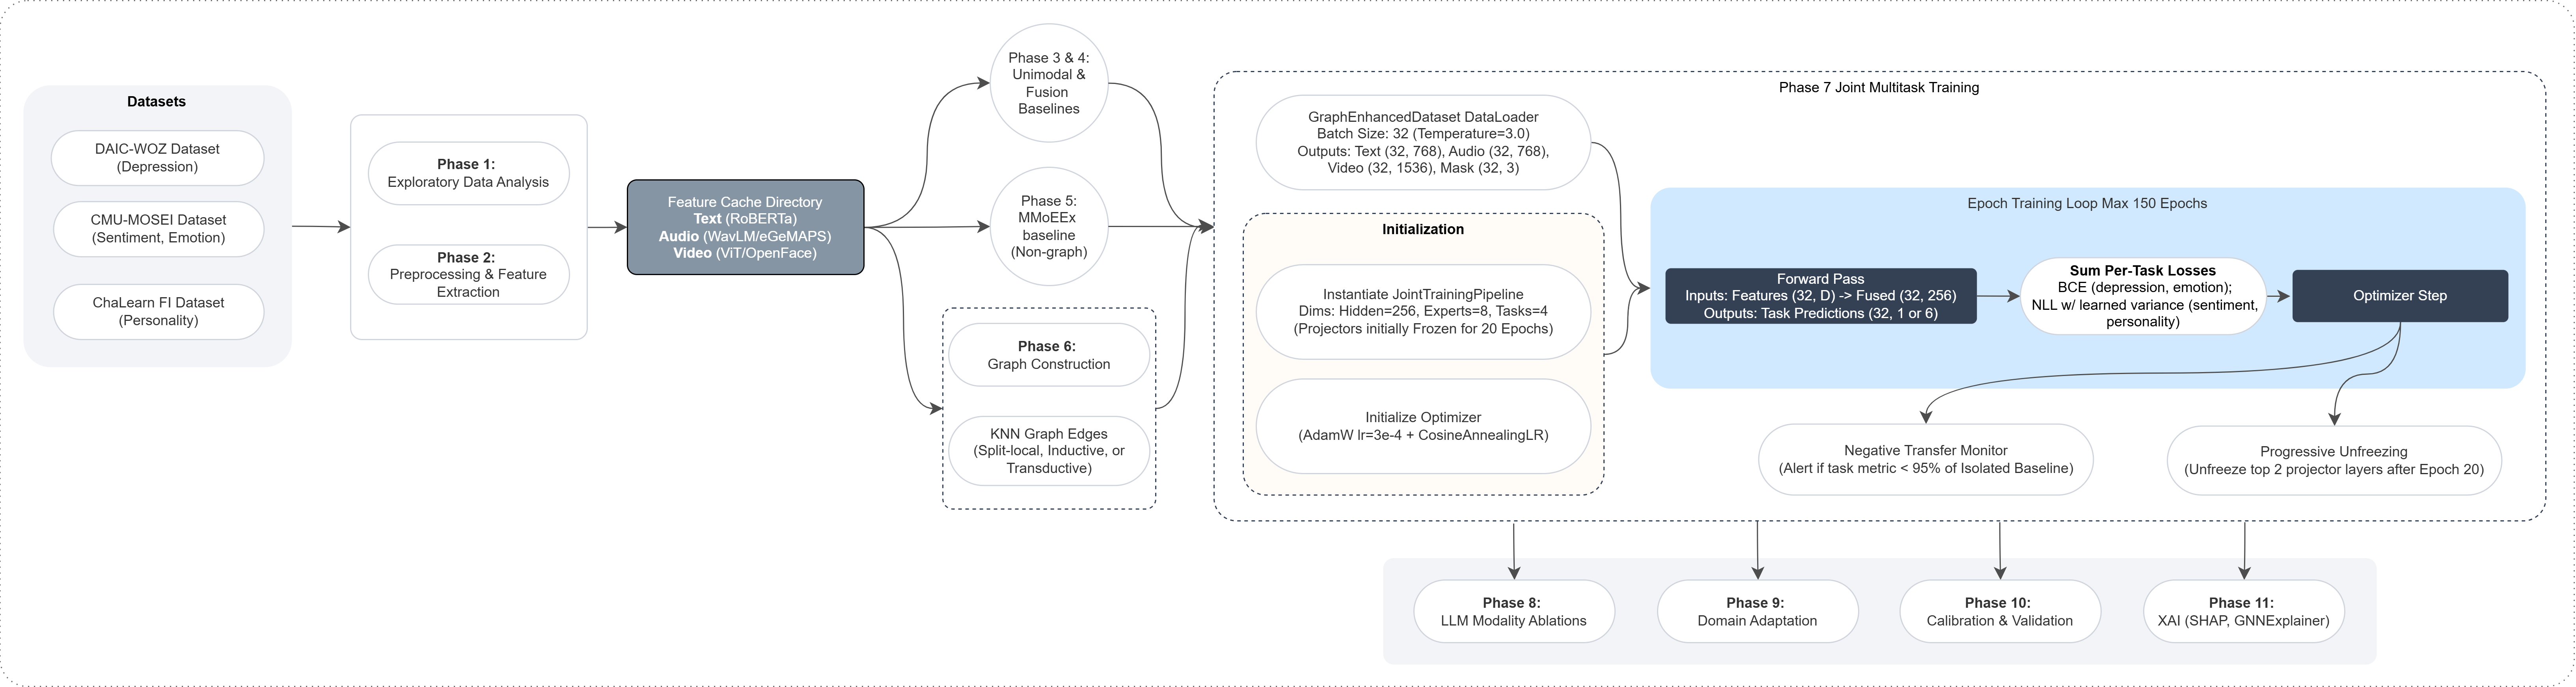
\includegraphics[width=0.85\textwidth]{figures/pipeline-flow.png}
\caption{Implementation detail of Phases 5--11: the non-graph MMoEEx baseline (Phase 5) and the graph-routed joint multitask training (Phase 7) share the same DataLoader, initialization, and epoch training loop, differing only in whether the graph router contributes to expert routing; downstream phases (LLM ablations, domain adaptation, calibration, explainability) follow.}
\label{fig:training_pipeline}
\end{figure*}

\section{Leakage Protocol Details}

\subsection{Graph Construction per Split}

For each dataset, we construct KNN graphs using one of three leakage-safe modes (see Section 3, ``Method,'' of the main paper):

\begin{itemize}
    \item \textbf{Inductive}: the graph is built on training-split embeddings only. Validation and test nodes connect exclusively to their $K$ nearest \emph{training} neighbours; they never connect to each other.
    \item \textbf{Split-local}: separate graphs are built independently for train, validation, and test. No edge crosses a split boundary.
    \item \textbf{Transductive} (ablation only, not leakage-safe): a single graph is built over all splits jointly, so validation/test nodes may connect to each other. Retained only to quantify how much a naive (non-leakage-safe) protocol would inflate results.
\end{itemize}

DAIC-WOZ: 189 sessions (107 train / 35 val / 47 test), subject-independent — no participant ID appears in more than one split. CMU-MOSEI and ChaLearn FI use their official utterance-/clip-level splits (see Section 3, ``Method,'' of the main paper). All splits are validated by an automated leakage audit (9/9 checks passing: inductive train/test, split-local val/test, transductive cross-split-edges-expected, bug-injection detection, and LLM-feature independence).

\section{Hyperparameters}

\begin{table}[t]
\centering
\caption{Complete hyperparameter configuration.}
\label{tab:hparams}
\small
\begin{tabular}{ll}
\toprule
Parameter & Value \\
\midrule
Common dimension $d$ & 256 \\
MMoEEx experts $M$ & 8 \\
Expert hidden size (both configurations) & 256 \\
GraphSAGE layers & 2 \\
GraphSAGE hidden size & 126 \\
GraphSAGE aggregation & Mean \\
GAT heads / head dim (ablation) & 3 / 42 \\
KNN neighbours $K$ & 10 or 15 (per variant) \\
Edge similarity metric & Cosine \\
Graph routing weight $\lambda$ & 0.5 (fixed, not tuned) \\
Learning rate & $3 \times 10^{-4}$ \\
Optimizer & AdamW \\
Batch size & 32 \\
Epochs (max) & 150 \\
Early stopping patience & 20 \\
Projector freeze epochs & 20 \\
Temperature balance $T$ & 3.0 \\
\bottomrule
\end{tabular}
\end{table}

\section{Complete Ablation Results}

\begin{table*}[t]
\centering
\caption{Full ablation ladder, real labels and real evaluation throughout. Each row adds one component cumulatively.}
\label{tab:full_ablation}
\small
\begin{tabular}{llcccc}
\toprule
 & & DAIC AUROC & MOSEI Sent. CCC & MOSEI Emotion AUROC & FI Avg CCC \\
\midrule
0 & Trivial (majority class) & 0.500 & 0.000 & 0.500 & 0.000 \\
1 & + Unimodal (best modality: text/text/video) & 0.671 & 0.512 & --$^\dagger$ & 0.458 \\
2 & + Gated late fusion & 0.442 & 0.575 & 0.634 & 0.000 \\
3 & + MMoEEx (no graph) & \textbf{0.573} & 0.493 & 0.703 & \textbf{0.571} \\
4 & + KNN voting (no learned router) & 0.630 & 0.443 & 0.676 & 0.390 \\
5 & + Graph router (V0, inductive $K{=}10$) & 0.489 & 0.486 & 0.713 & 0.519 \\
6 & + Graph router (V3, inductive $K{=}15$) & 0.533 & \textbf{0.508} & \textbf{0.720} & 0.531 \\
\bottomrule
\end{tabular}

\vspace{2pt}
{\footnotesize $^\dagger$Per-modality unimodal baselines evaluate MOSEI emotion as a regression task (CCC per emotion, averaged); no per-modality classification AUROC was computed at the unimodal stage, so this cell is not directly comparable to the classification AUROC reported for rows 2--6 and is left blank rather than filled with an unrelated number.}
\end{table*}

Row 4 (simple KNN label voting, no learned GraphSAGE router at all) reaches the best DAIC AUROC in the entire ladder except for row 3, the non-graph MMoEEx baseline (0.573) — which an earlier version of this table understated as chance-level (0.493) due to a temperature-balanced-sampling bug (\S\ref{sec:xai_supp} and main paper, Section~4) that let MOSEI's $\sim$32k task-rows swamp DAIC's 107 training rows in nearly every batch. With that fixed, the non-graph baseline is the best DAIC AUROC in the ladder, and the learned graph router (rows 5--6) underperforms both it and the simple KNN heuristic (row 4) — the clearest single illustration that the learned component fails to add value over either a working non-graph baseline or the simplest graph-based heuristic on the primary clinical task.

\section{Graph-Sensitivity Sweep}

\begin{figure}[t]
\centering

\includegraphics[width=0.9\columnwidth]{figures/k_sensitivity.png}
\caption{No monotonic trend with $K \in \{5,10,15,20\}$ (inductive graph): DAIC AUROC is 0.496, 0.489, 0.533, 0.449 respectively, none reaching the 0.573 non-graph baseline. $K{=}20$ is the worst configuration, below chance.}
\label{fig:k_sensitivity}
\end{figure}

\section{Learned Routing Weight}

\begin{figure}[t]
\centering
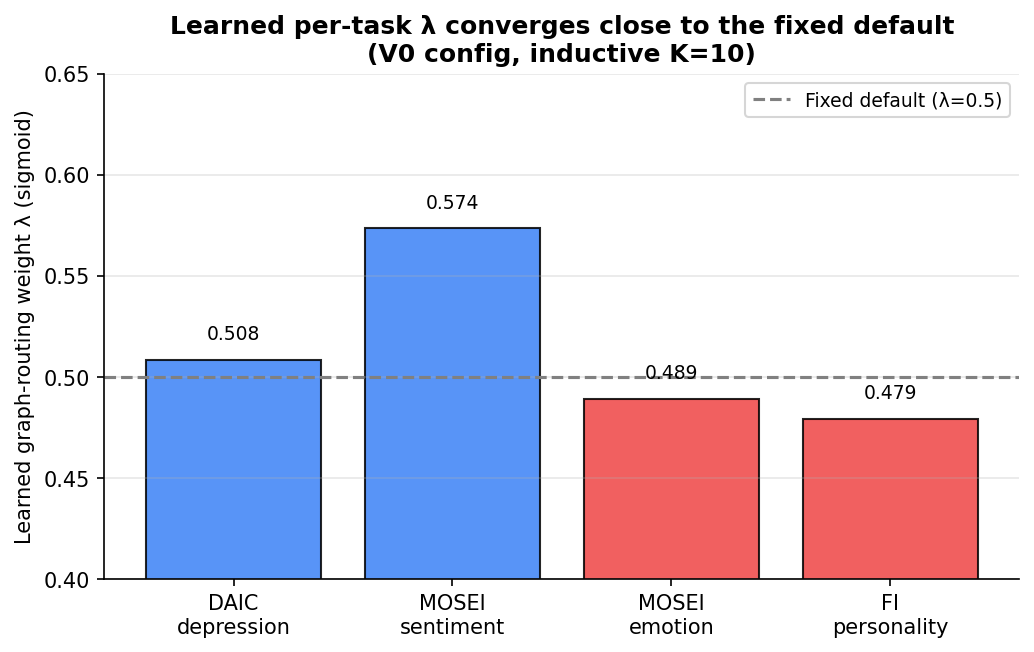
\includegraphics[width=0.9\columnwidth]{figures/learned_lambda.png}
\caption{Learned per-task $\lambda$ (V0 configuration, values 0.479--0.574) vs.\ the fixed default (0.5): a real gain on DAIC (AUROC 0.489 $\to$ 0.525, still short of the 0.573 non-graph baseline) but not on FI (CCC 0.519 $\to$ 0.503, moving further from the 0.571 baseline).}
\label{fig:learned_lambda}
\end{figure}

\section{Additional Figures}

\begin{figure}[t]
\centering
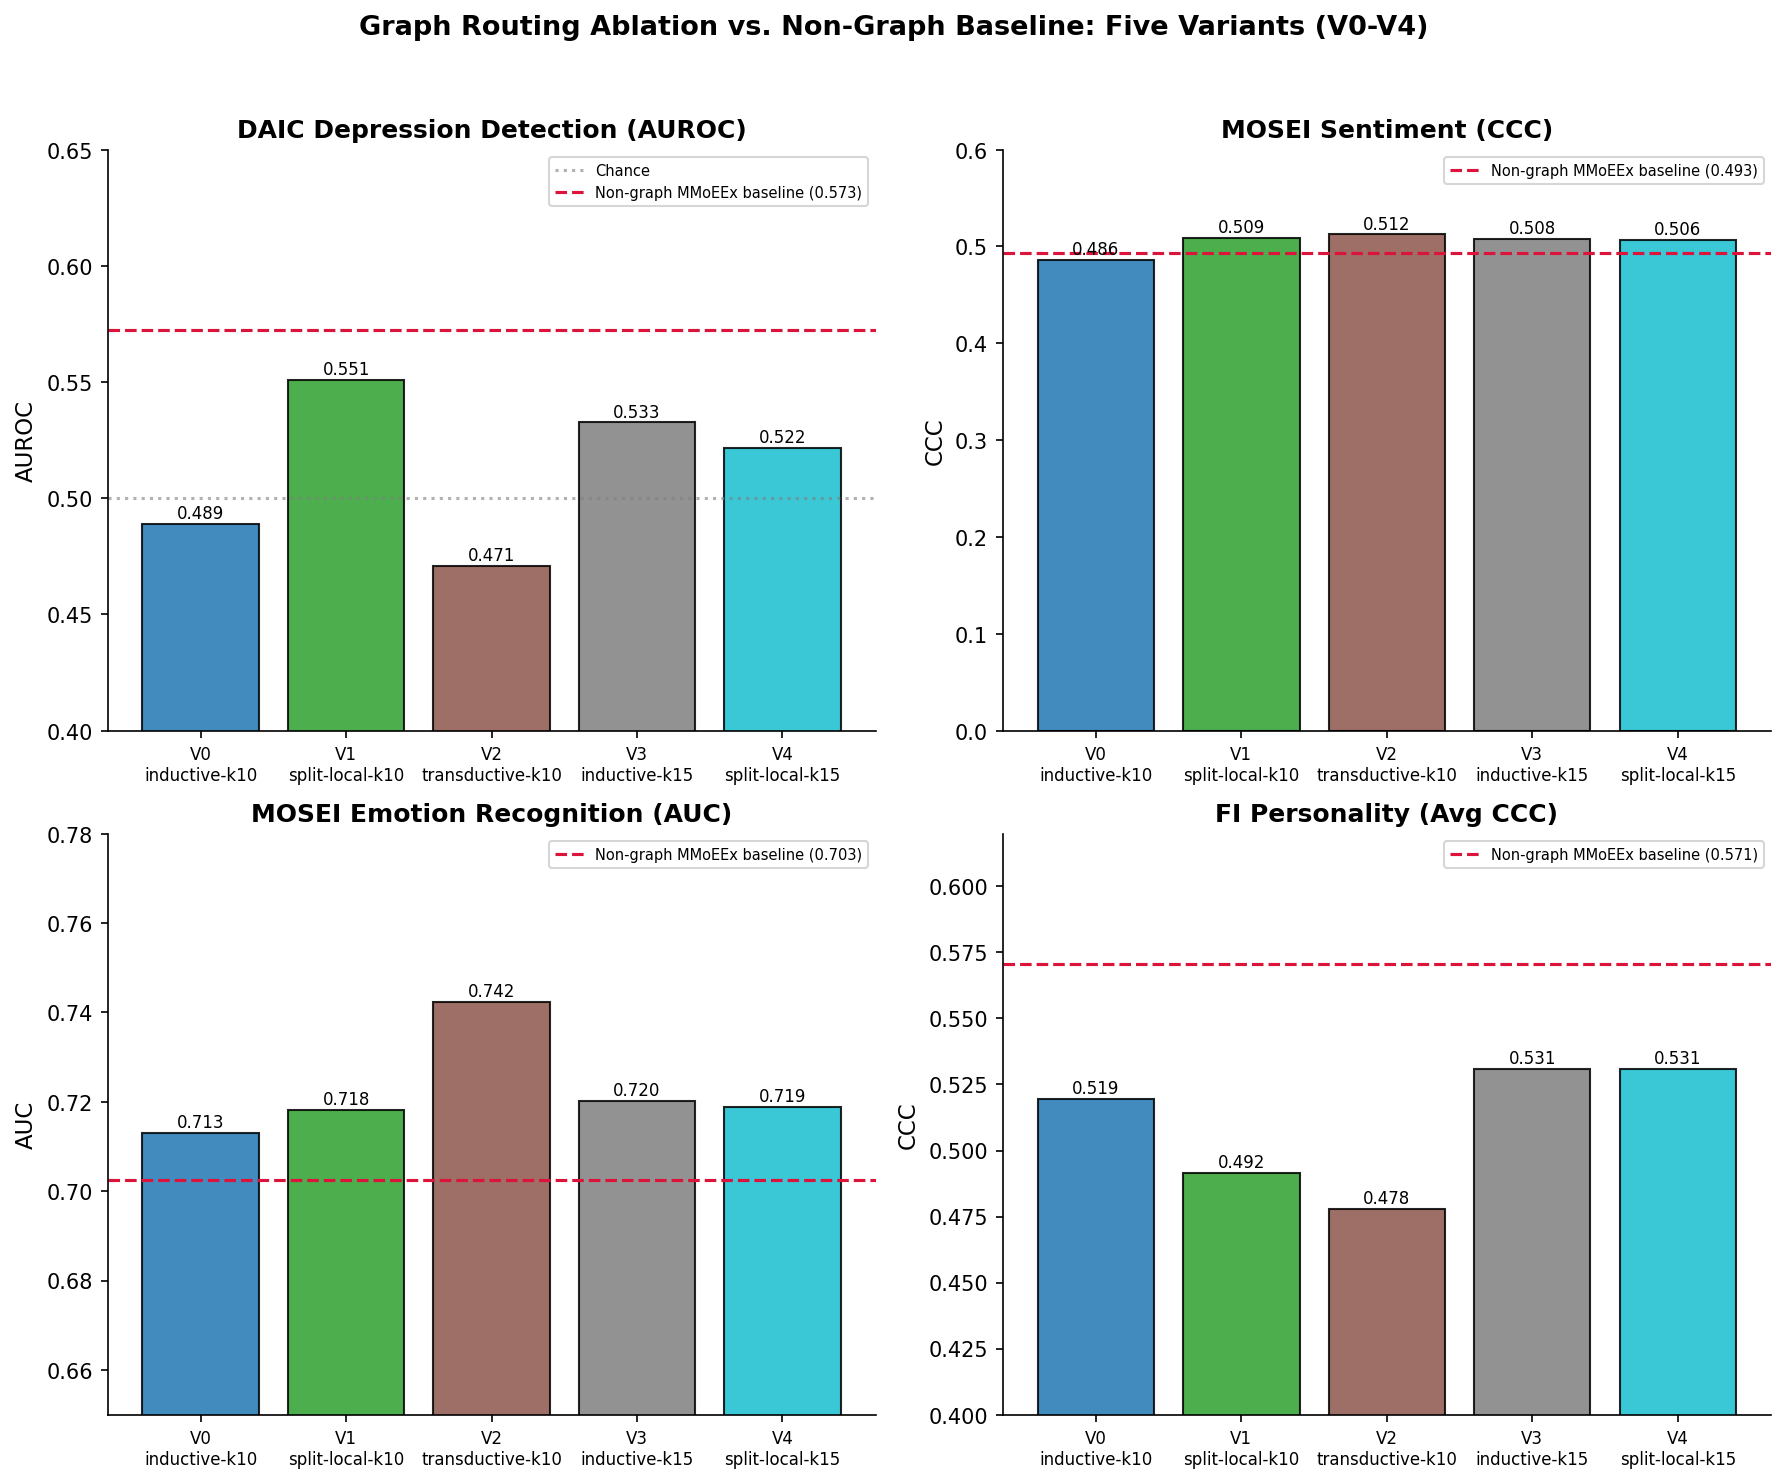
\includegraphics[width=0.9\columnwidth]{figures/graph_ablation.png}
\caption{Graph routing ablation vs.\ non-graph MMoEEx baseline (red dashed line), all five variants across all four tasks.}
\label{fig:graph_ablation_supp}
\end{figure}

\begin{figure}[t]
\centering
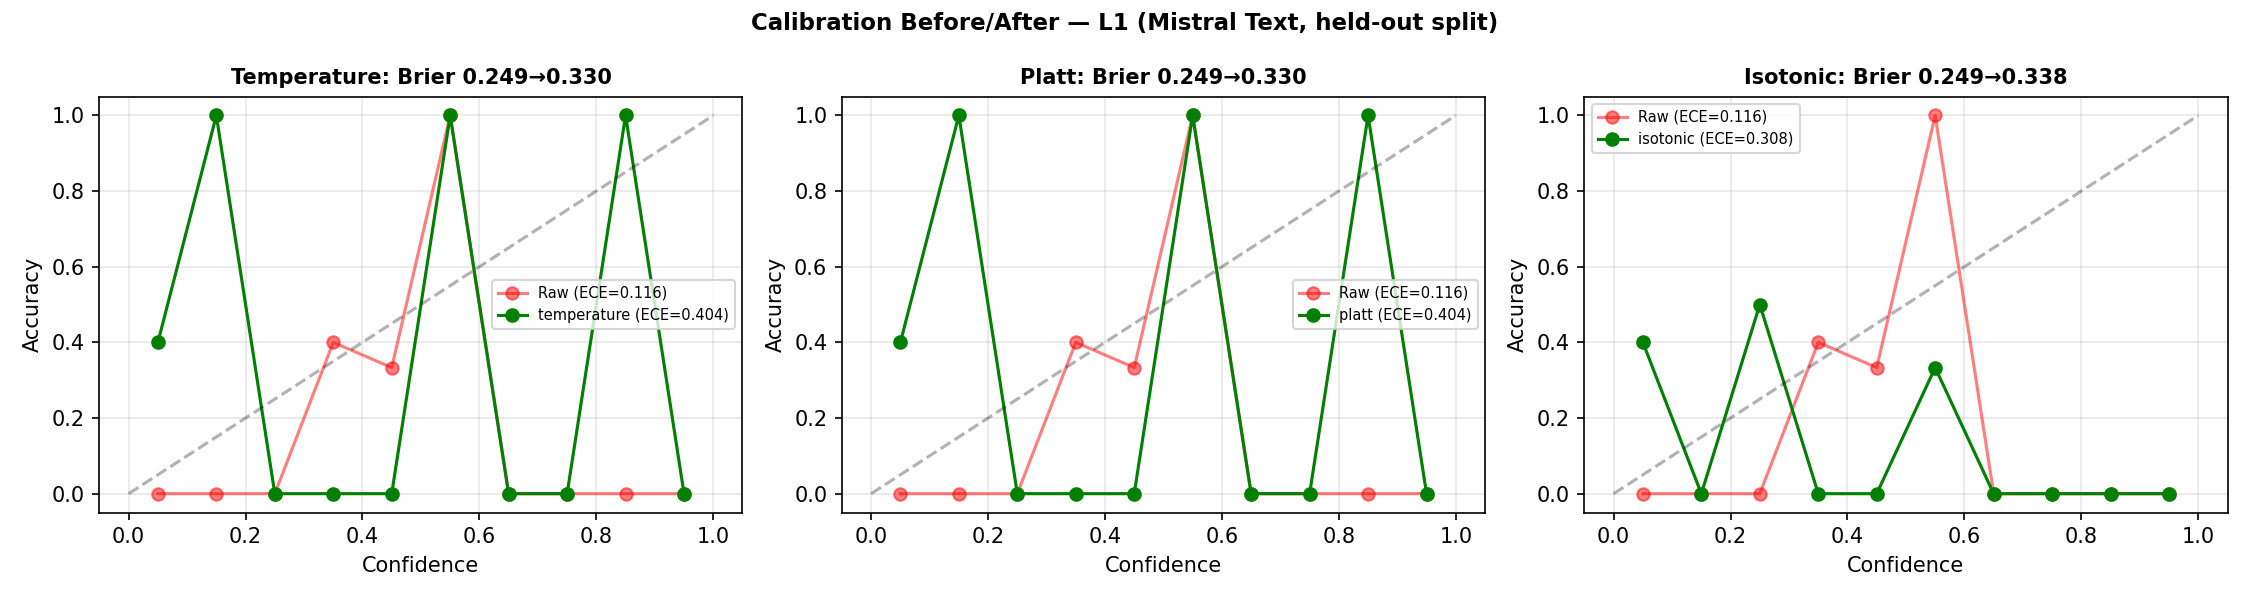
\includegraphics[width=0.9\columnwidth]{figures/calibration.png}
\caption{Calibration reliability diagrams (temperature/Platt/isotonic scaling vs.\ raw) for the L1 (Mistral text) DAIC depression classifier, held-out split. Monotonic recalibration changes reliability (ECE/Brier) but not ranking-based discrimination (AUROC), since AUROC is invariant to monotonic transforms of the score.}
\label{fig:calibration}
\end{figure}

\section{Domain Adaptation Detail}
\label{sec:domain_adaptation_supp}

We tested unsupervised domain adaptation (CORAL, MMD, DANN, and a combined CORAL+MMD loss) for transferring FI and MOSEI representations to DAIC depression detection, against a no-adaptation baseline, across three transfer scenarios (FI$\to$DAIC, MOSEI$\to$DAIC, multisource). All four methods underperform the no-adaptation baseline in 10 of 12 evaluated conditions: the no-adaptation baseline's best result (MOSEI$\to$DAIC, AUROC=0.6942) beats the best DA result anywhere (combined CORAL+MMD, FI$\to$DAIC, AUROC=0.6901); CORAL is the most consistently harmful ($-$0.0744 vs.\ baseline at worst), and only MMD marginally improves its own no-adaptation baseline (+0.0041, within bootstrap CI). We attribute this to DAIC's training set ($n{=}107$) being too small to train a stable domain discriminator, and to shared multitask heads already providing implicit alignment; we do not merge domain adaptation into the main model.

\section{MPDD Cross-Dataset Generalization Detail}
\label{sec:mpdd_supp}

To probe whether our findings generalize beyond DAIC/MOSEI/FI, we ran a supplementary benchmark on MPDD (Multimodal Depression Detector: Wav2Vec2 + OpenFace features, two age tracks). On MPDD-Young, a strongly-regularized logistic regression (AUROC=0.674) outperforms both GGMoE with and without graph routing (0.545/0.559) — the small sample size favors a linear model over any neural architecture we tested, including the graph router.

\begin{figure}[t]
\centering
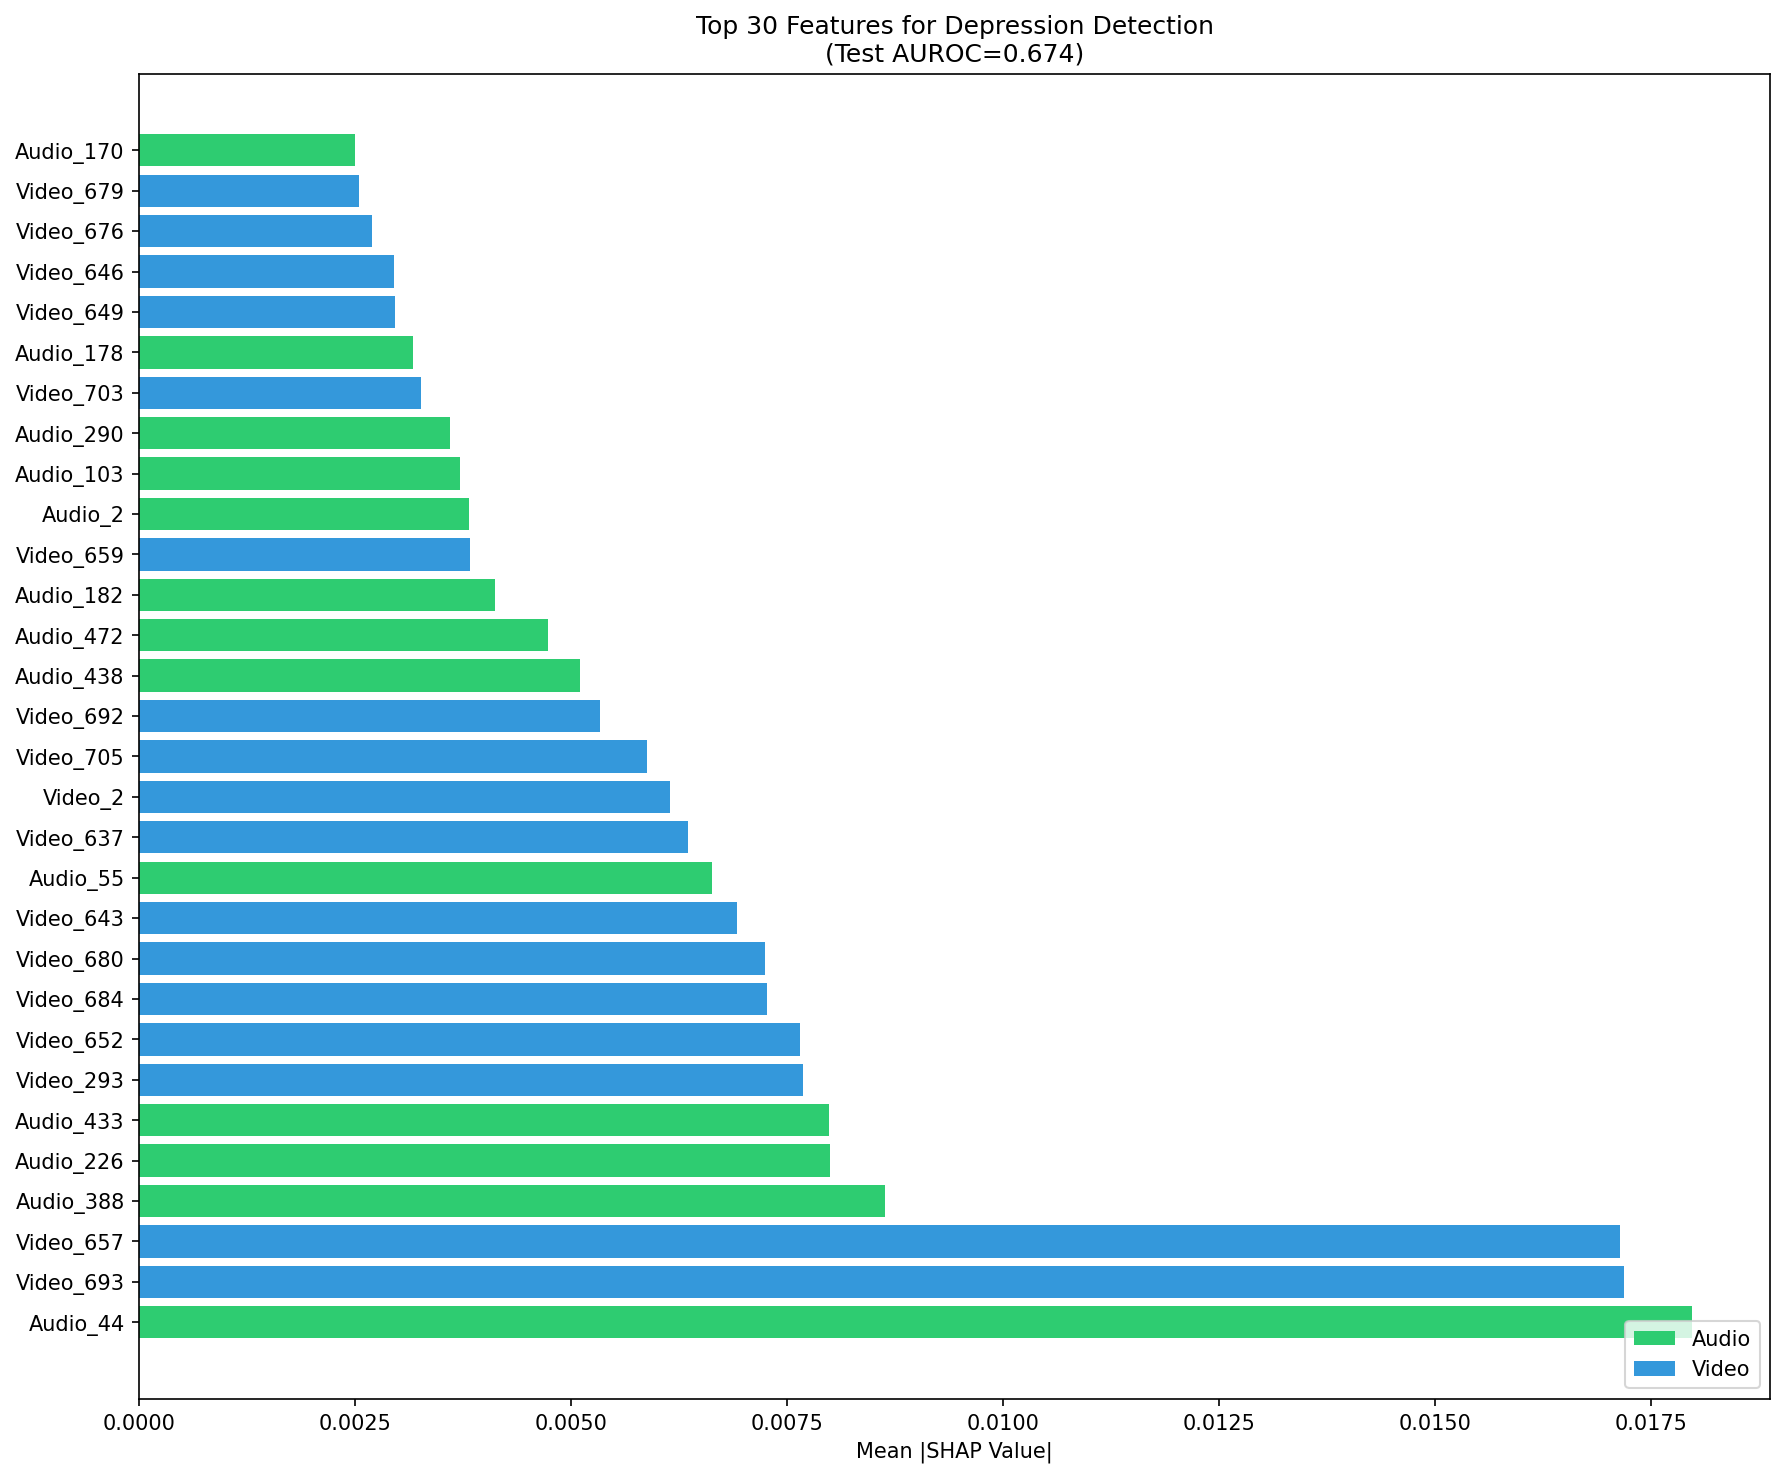
\includegraphics[width=0.9\columnwidth]{figures/feature_importance.png}
\caption{Top-30 SHAP feature importances for MPDD-Young depression detection. \texttt{audio\_44} is the single most important feature, though the top-30 set is video-dominated (17 of 30).}
\label{fig:mpdd_shap_supp}
\end{figure}

Zero-shot transfer from Young to Elderly collapses to near-constant predictions (cross-track AUROC=0.395, below chance), while cross-\emph{dataset} transfer sharing a Wav2Vec2-family audio encoder (MPDD$\to$DAIC) transfers positively (AUROC=0.551, above the within-DAIC baseline of 0.344) — encoder-family match appears to matter more than domain similarity for transfer, and age-group-specific rather than universal biomarkers likely explain the cross-track failure.

\section{Expert Routing Analysis}

Figure~\ref{fig:expert_distribution} shows the real MMoEEx routing-weight distribution (non-graph baseline): each task concentrates weight on a small subset of its assigned experts rather than routing uniformly, indicating the gates learn task-differentiated behaviour even where the aggregate metric for that task declines relative to a unimodal baseline (see main paper).

\begin{figure}[t]
\centering
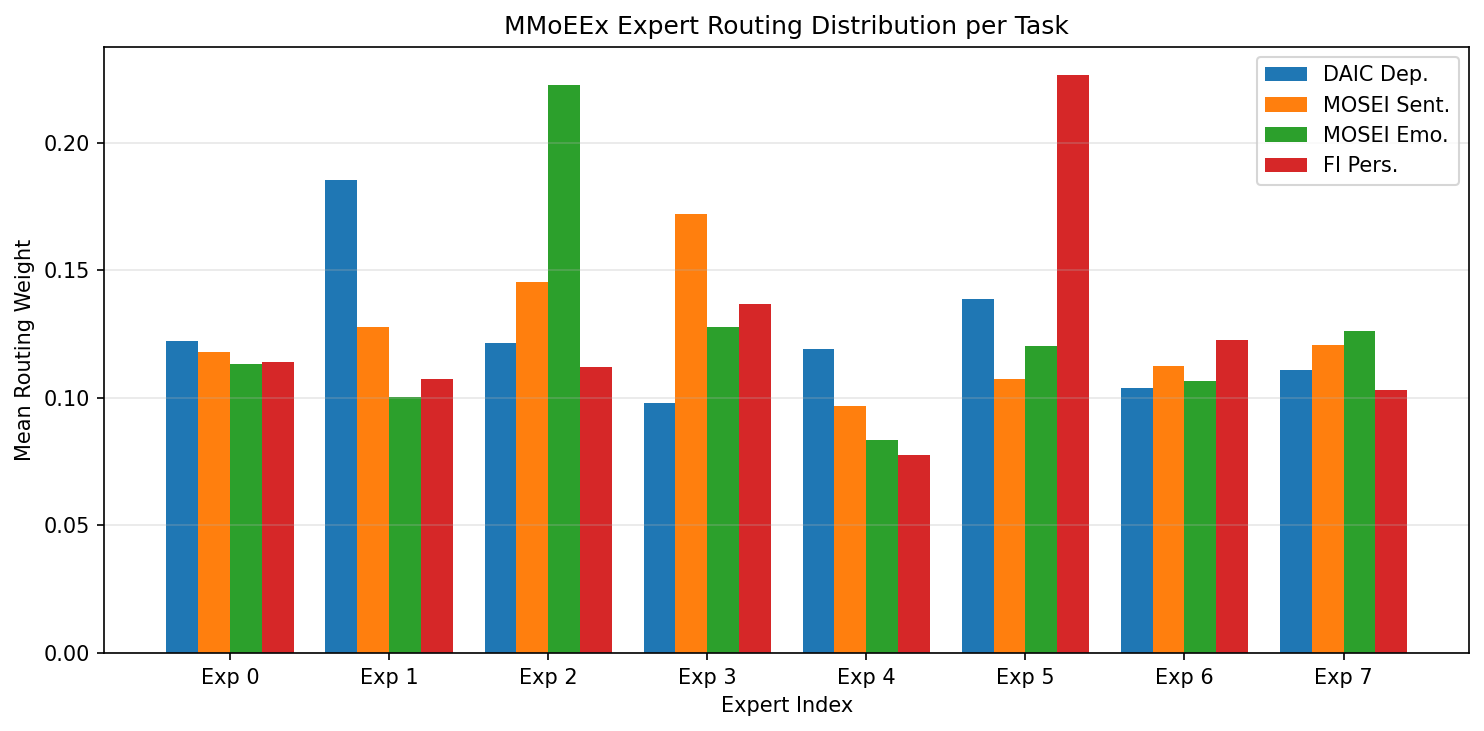
\includegraphics[width=0.9\columnwidth]{figures/expert_distribution.png}
\caption{Mean MMoEEx routing weight per expert and task (non-graph baseline). Rows/legend are tasks; columns are the 8 experts.}
\label{fig:expert_distribution}
\end{figure}

\section{Explainability Case Studies}
\label{sec:xai_supp}

Beyond the routing-performance question, the main paper's Introduction motivates two further, separately-evaluated hypotheses: that mental health assessment can be made more transparent by characterizing depression jointly with sentiment, emotion, and personality rather than in isolation, and that a graph over similar individuals can give both a visual and a machine-readable account of what informed a prediction. This section reports both.

\subsection{Multi-Construct Characterization}

For 9 case studies (3 per dataset), we pass the same sample's shared representation through all four task heads — not only the head matching its own source dataset — producing a depression probability, sentiment score, six emotion probabilities, and five personality-trait scores for the same person in one forward pass. On a representative positive-sentiment MOSEI case, the profile is internally coherent: happiness probability 0.89, sentiment score $+0.62$, with sadness/anger/fear all below 0.09 — a plausible joint characterization rather than four unrelated numbers. Related work explicitly separating personality-trait context from acute depression symptoms in an interpretable graph model \citep{vyalla2026psygat} supports this direction; each profile is stored as a \texttt{multi\_construct\_profile} field in \texttt{artifacts/tables/phase11\_xai\_results.json}.

\subsection{Graph-Based Explanation}

For each case study we generate a visual record (SHAP per-modality beeswarm plot, GNNExplainer-style subgraph diagram \citep{gnnexplainer2019}, and a GraphXAIN-style \citep{cedro2024graphxain} natural-language narrative panel, Figure~\ref{fig:graphxain_supp}) and a machine-readable record (SHAP values, top-$k$ neighbour identities and cosine distances, expert routing weights, the multi-construct profile, and counterfactual/perturbation deltas). The narrative is generated by prompting an LLM (Mistral-7B) with the SHAP values, subgraph structure, and sample metadata, used purely as \emph{post-hoc} explanation of an independently-computed prediction — not as reasoning inserted into the prediction pipeline itself. This distinction matters: chain-of-thought-style reasoning improves mental-health text classification when used to produce the prediction \citep{patil2025cognitivemental}, but can be unfaithful or reduce reliability when embedded in the clinical decision itself \citep{wu2025cotfails}.

\begin{figure}[t]
\centering
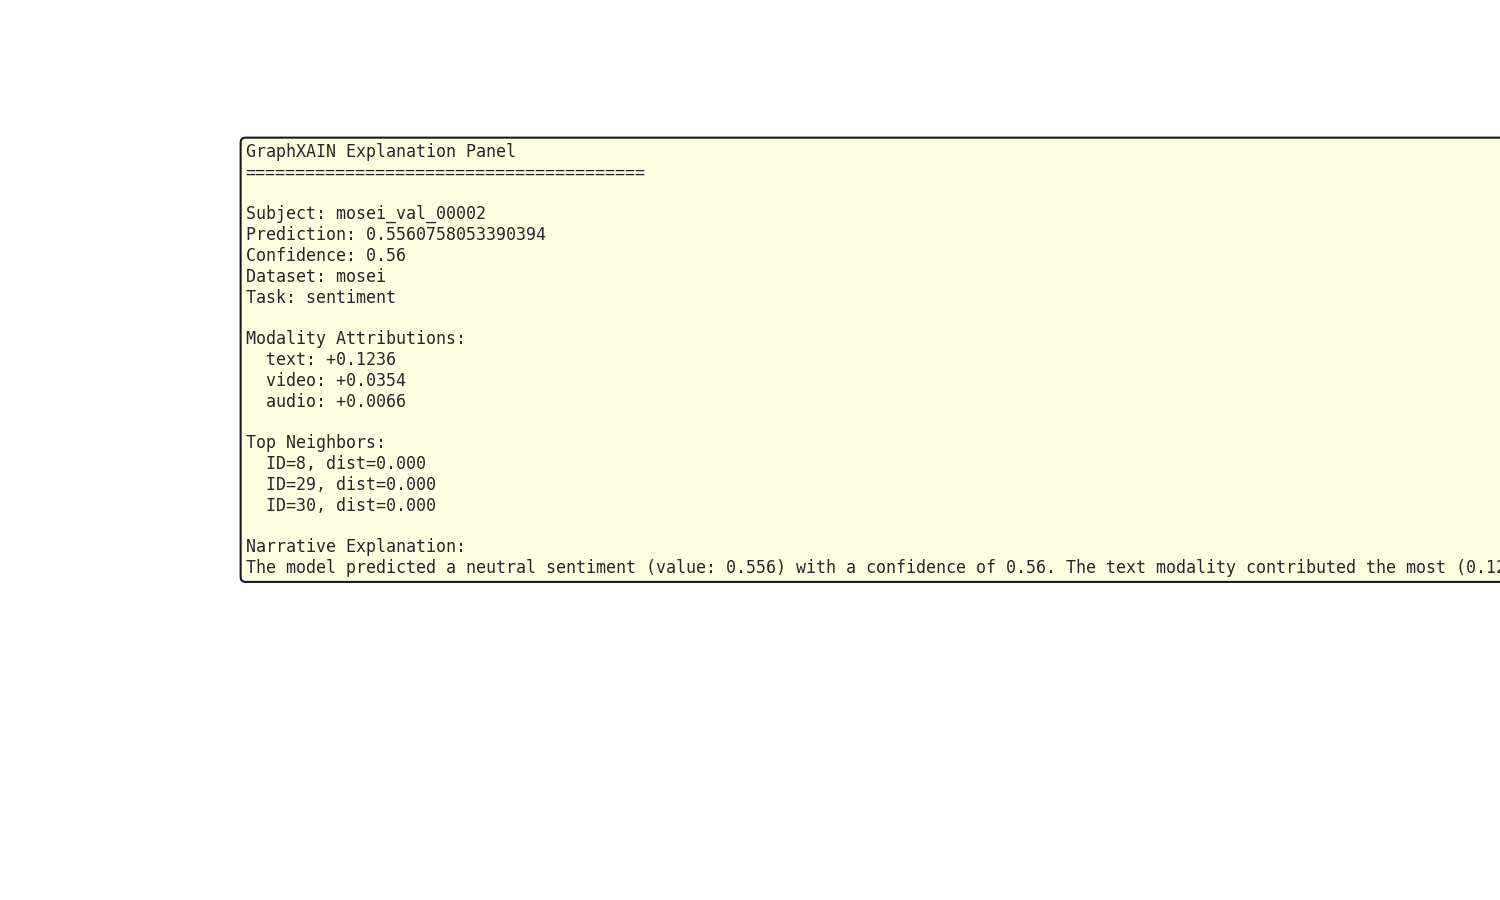
\includegraphics[width=0.9\columnwidth]{../artifacts/figures/phase_11_xai/mosei_graphxain_panel.png}
\caption{GraphXAIN-style narrative panel for a representative MOSEI case, combining SHAP attribution, subgraph structure, and sample metadata into a post-hoc natural-language explanation.}
\label{fig:graphxain_supp}
\end{figure}

Every SHAP, perturbation, and counterfactual value must be computed under each sample's own dataset-native routing (main paper, Section 3): DAIC is evaluated text-only and FI video-only, so a modality outside a dataset's native routing shows \emph{exactly} zero attribution, not a small residual. Across 90 perturbation tests, only 47 are non-zero, exactly matching each sample's routing; the remaining 43 are exactly zero rather than merely small. This is a stronger faithfulness check than a ranking comparison: it directly confirms the explanation pipeline reflects each dataset's real computation.

\begin{figure}[t]
\centering
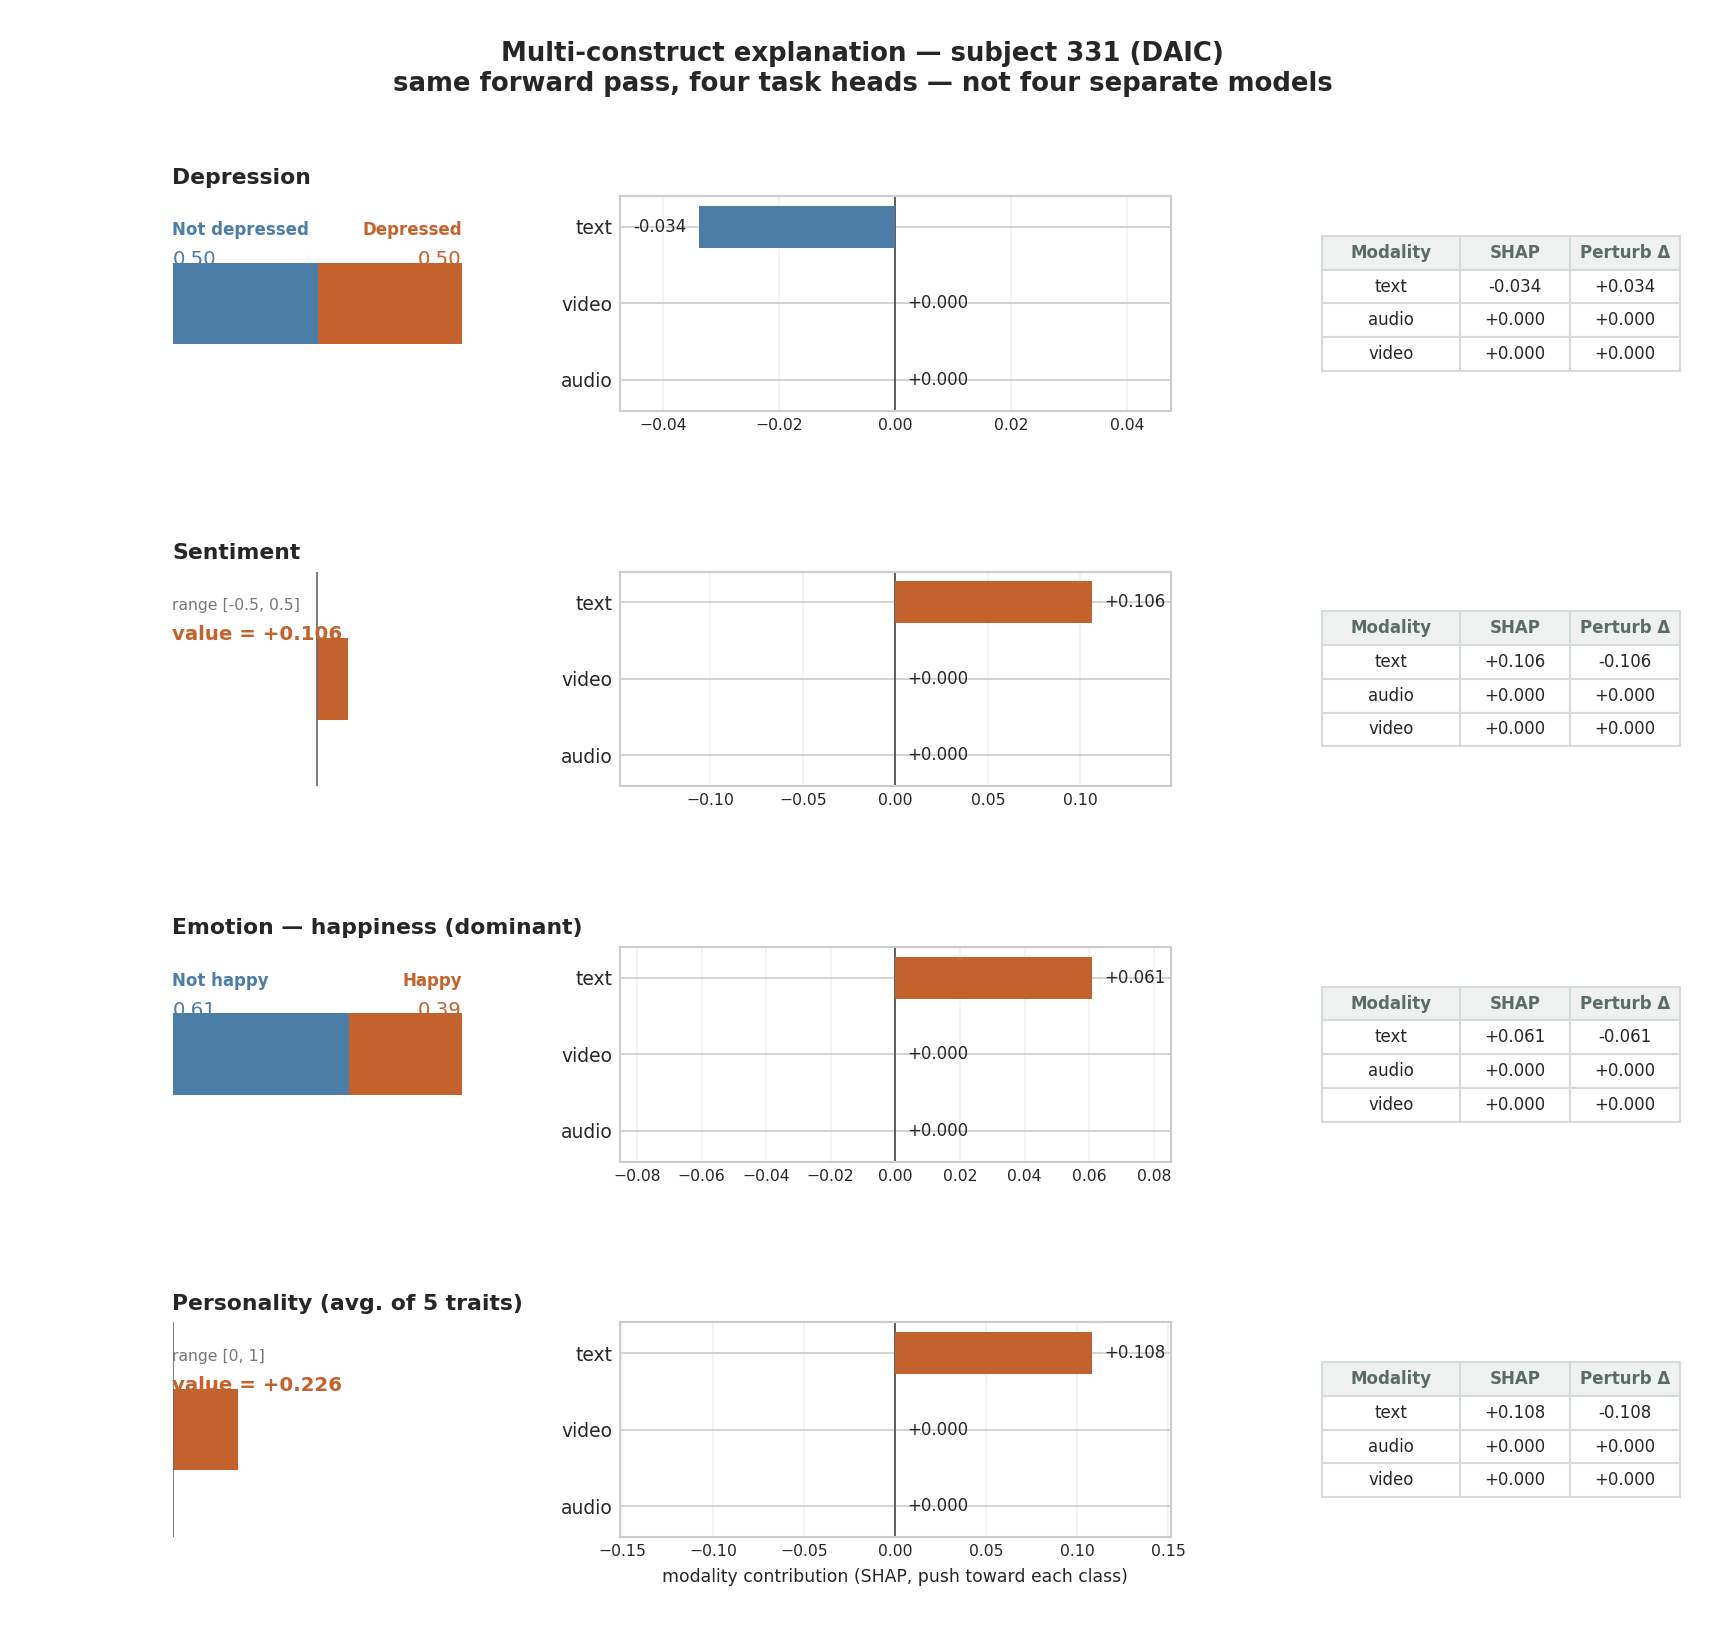
\includegraphics[width=0.9\columnwidth]{../artifacts/figures/phase_11_xai/daic_multi_construct_force.png}
\caption{Multi-construct force plot: one DAIC subject explained through all four task heads in a single figure. Audio and video read exactly zero on every row, visualizing DAIC's text-only routing directly rather than leaving it implicit.}
\label{fig:force_panel_supp}
\end{figure}

The explanation graph is built on the model's own trained fused representation rather than raw concatenated features, so reported neighbours are the ones the router and task heads actually operate on. This does not, however, improve DAIC label homophily: on the same 35 DAIC validation samples used for the main paper's homophily diagnostic, label agreement is 0.577 for raw features, 0.537 for random pairing, and 0.463 (below random) for the trained representation, since task-supervised training optimizes for the final decision boundary rather than for preserving neighbourhood structure. DAIC subgraph explanations should be read as faithful to the model's own computation, without a validated claim that the shown neighbours are similar in a depression-relevant sense; MOSEI and FI do not share this limitation, consistent with the main paper's homophily diagnostic finding real label signal for those tasks.

\bibliography{references/references}
\end{document}
